%%%%%%%%%%%%%%%%%%%%%%%%%%%%%%%%%%%%%%%%%
% Short Sectioned Assignment LaTeX Template Version 1.0 (5/5/12)
% This template has been downloaded from: http://www.LaTeXTemplates.com
% Original author:  Frits Wenneker (http://www.howtotex.com)
% License: CC BY-NC-SA 3.0 (http://creativecommons.org/licenses/by-nc-sa/3.0/)
%%%%%%%%%%%%%%%%%%%%%%%%%%%%%%%%%%%%%%%%%

%----------------------------------------------------------------------------------------
%	PACKAGES AND OTHER DOCUMENT CONFIGURATIONS
%----------------------------------------------------------------------------------------

\documentclass[paper=a4, fontsize=11pt]{scrartcl} % A4 paper and 11pt font size

% ---- Entrada y salida de texto -----

\usepackage{hyperref}
\usepackage{varioref}
\usepackage[T1]{fontenc} % Use 8-bit encoding that has 256 glyphs
\usepackage[utf8]{inputenc}
%\usepackage{fourier} % Use the Adobe Utopia font for the document - comment this line to return to the LaTeX default

% ---- Idioma --------

\usepackage[spanish, es-tabla]{babel} % Selecciona el español para palabras introducidas automáticamente, p.ej. "septiembre" en la fecha y especifica que se use la palabra Tabla en vez de Cuadro

% ---- Otros paquetes ----

\usepackage{amsmath,amsfonts,amsthm} % Math packages
%\usepackage{graphics,graphicx, floatrow} %para incluir imágenes y notas en las imágenes
\usepackage{graphics,graphicx, float} %para incluir imágenes y colocarlas

% Para hacer tablas comlejas
%\usepackage{multirow}
%\usepackage{threeparttable}

%\usepackage{sectsty} % Allows customizing section commands
%\allsectionsfont{\centering \normalfont\scshape} % Make all sections centered, the default font and small caps

\usepackage{fancyhdr} % Custom headers and footers
\pagestyle{fancyplain} % Makes all pages in the document conform to the custom headers and footers
\fancyhead{} % No page header - if you want one, create it in the same way as the footers below
\fancyfoot[L]{} % Empty left footer
\fancyfoot[C]{} % Empty center footer
\fancyfoot[R]{\thepage} % Page numbering for right footer
\renewcommand{\headrulewidth}{0pt} % Remove header underlines
\renewcommand{\footrulewidth}{0pt} % Remove footer underlines
\setlength{\headheight}{13.6pt} % Customize the height of the header

\numberwithin{equation}{section} % Number equations within sections (i.e. 1.1, 1.2, 2.1, 2.2 instead of 1, 2, 3, 4)
\numberwithin{figure}{section} % Number figures within sections (i.e. 1.1, 1.2, 2.1, 2.2 instead of 1, 2, 3, 4)
\numberwithin{table}{section} % Number tables within sections (i.e. 1.1, 1.2, 2.1, 2.2 instead of 1, 2, 3, 4)

\setlength\parindent{0pt} % Removes all indentation from paragraphs - comment this line for an assignment with lots of text

\newcommand{\horrule}[1]{\rule{\linewidth}{#1}} % Create horizontal rule command with 1 argument of height


 \usepackage{algpseudocode}
%----------------------------------------------------------------------------------------
%	TÍTULO Y DATOS DEL ALUMNO
%----------------------------------------------------------------------------------------

\title{	
\normalfont \normalsize 
\textsc{{\bf Ing. del Conocimiento (2015-2016)} \\ Grado en Ingeniería Informática \\ Universidad de Granada} \\ [25pt] % Your university, school and/or department name(s)
\horrule{0.5pt} \\[0.4cm] % Thin top horizontal rule
\huge Sistema Experto En Bolsa \\ % The assignment title
\horrule{2pt} \\[0.5cm] % Thick bottom horizontal rule
}

\author{Francisco Carrillo Pérez \\DNI: 77140580-Y} % Nombre y apellidos

\date{\normalsize\today} % Incluye la fecha actual

%----------------------------------------------------------------------------------------
% DOCUMENTO
%----------------------------------------------------------------------------------------

\begin{document}

\maketitle % Muestra el Título

\newpage %inserta un salto de página

\tableofcontents % para generar el índice de contenidos

\listoffigures

\newpage

\section{Introducción }

En este documento se van a tratar los distintos aspectos que han tenido que ver con la realización de un sistema experto para el apoyo en inversión bursátil, realizado con la herramienta CLIPS.
%----------------------------------------------------------------------------------------
\section{Resumen del funcionamiento del sistema experto}
El funcionamiento del sistema experto es el siguiente:
\begin{enumerate}
	\item Se cargan los datos, que se leen desde los ficheros de texto \textit{Analisis.txt},\textit{AnalisisSectores.txt}, \textit{Cartera.txt} y \textit{Noticias.txt}. En ellos se encuentran todos los datos requeridos por el sistema experto.
	\item Se procede a la detección del tipo de valores que tenemos, dentro de los cuáles podemos tener: \textit{valores inestables}, \textit{valores peligrosos}, \textit{valores sobrevalorados} y \textit{valores infravalorados}.
	\item Con estos datos, se pasa al módulo de realización de propuestas.
	\item Una vez que se han obtenido todas las propuestas posibles, se muestran al usuario las 5 mejores, y si hay menos de 5 entonces todas las que sean, y se le pide que elija una, introduciéndo el número de la propuestas que se observa por pantalla.También puede elegir no hacer nada, en ese caso la ejecución terminaría.
	\item Según la propuesta elegida,se pide la cantidad de acciones con las que se desea trabajar y se aplican los cambios sobre la cartera del usuario y se vuelve al módulo de realización de propuestas.Como he indicado anteriormente, el usuario puede parar la ejecución decidiéndo no aceptar ninguna propuesta.
\end{enumerate}
Podemos observar unas imágenes de la ejecución acontinuación: \\
\begin{figure}[H]
	\centering
	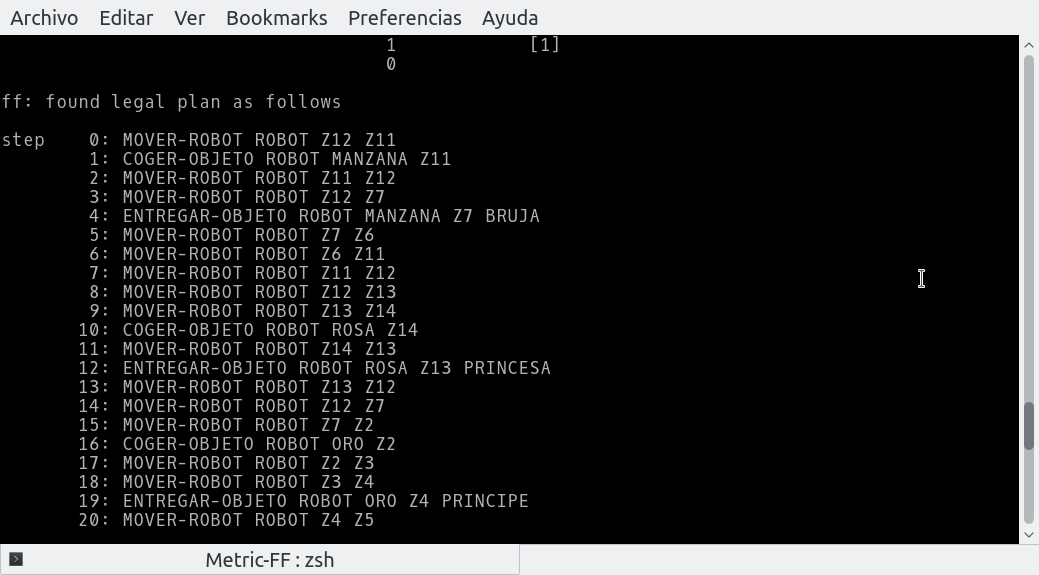
\includegraphics[width=0.8\textwidth]{img1.png}
	\caption{Inicio del sistema experto}
	\label{fig:iniciodelsistema}
\end{figure}
\begin{figure}[H]
	\centering
	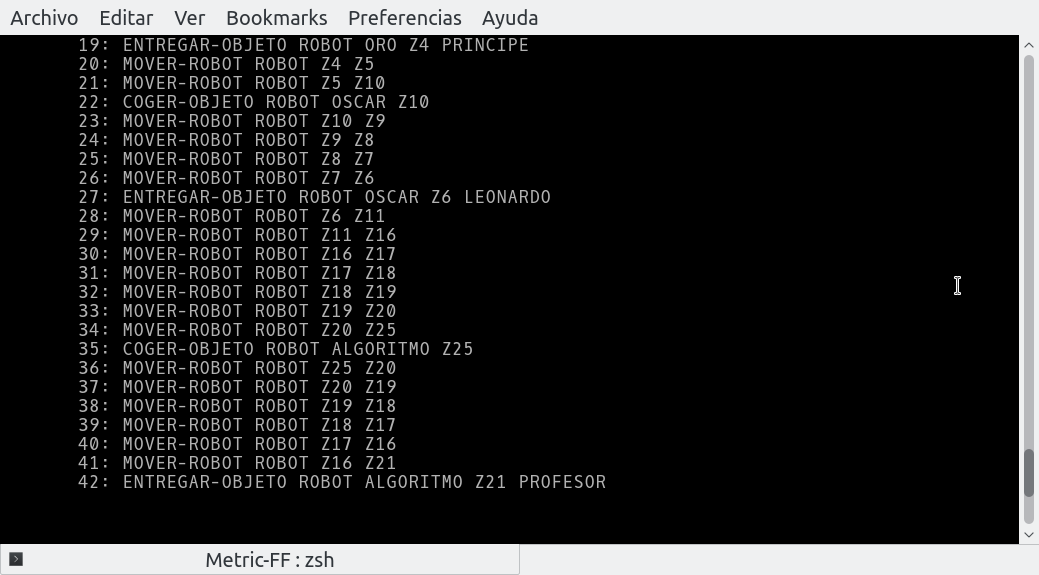
\includegraphics[width=0.8\textwidth]{img2.png}
	\caption{Ejemplo propuesta del sistema experto}
	\label{fig:propuesta}
\end{figure}
\begin{figure}[H]
	\centering
	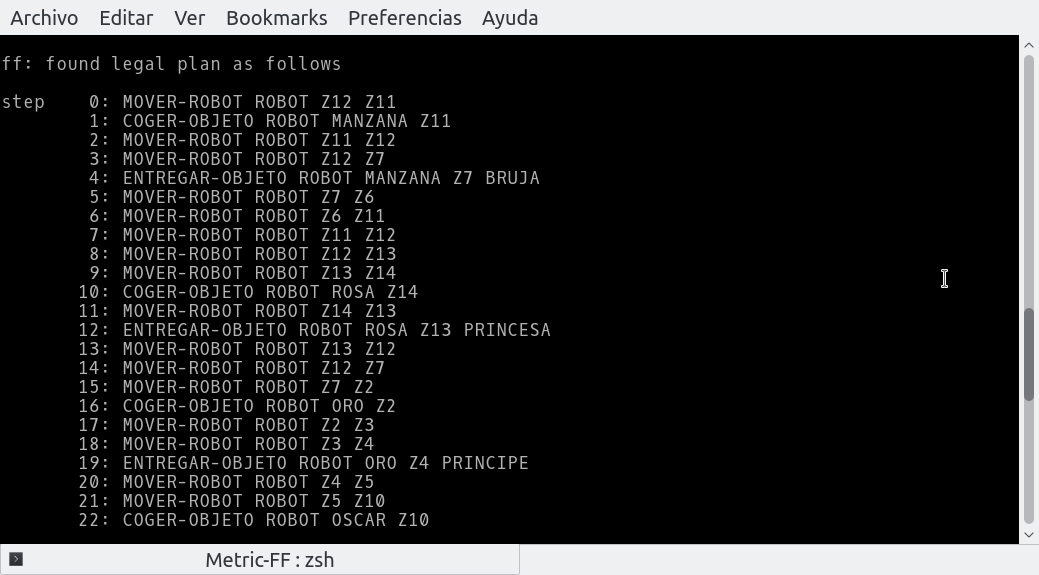
\includegraphics[width=0.8\textwidth]{img3.png}
	\caption{Ejemplo propuesta de venta del sistema experto}
	\label{fig:cantidad}
\end{figure}

\section{Descripción del proceso seguido para el desarrollo}
Para el desarrollo se ha utilizado la información obtenida en las distintas sesiones con el experto realizadas durante las clases de teoría de la asignatura, además de las clases de prácticas en las que también se realizaron sesiones. El resto de conocimiento se ha obtenido del PDF \textit{conocimiento.pdf}.\\
Para el proceso de validación y verificación se ha comprobado con distintas entradas,es decir, con los valores de distintos días para comprobar si realizando el proceso,como quedaba la base de hechos(consultándola con el comando \textit{(facts)}) se correspondía a lo que debía ser, además de que se realizaban los cambios correctamente.

\section{Descripción del sistema desarrollado }
\subsection{Conocimiento global del sistema}
En el sistema al comienzo se cargan los datos de las siguientes fuentes que se han comentado en la sección 2:
\begin{itemize}
	\item \textit{Analisis.txt}: Los datos de esta fuente se insertaran en hechos con el template \textbf{Empresa}, el cuál se ha comentado en la subsección anterior.
	\item \textit{AnalisisSectores.txt}: Los datos de esta fuente se insertaran en hechos con el template \textbf{Sector}, el cuál se ha comentado en la subsección anterior.
	\item \textit{Noticias.txt}: Los datos de esta fuente se insertaran en hechos con el template \textbf{Noticia}, el cuál se ha comentado en la subsección anterior.
	\item \textit{Cartera.txt}: Los datos de esta fuente se insertaran en hechos con los template \textbf{Cartera} y \textbf{PrimeraLinea}, los cuáles se han comentado en la subsección anterior.	
\end{itemize}
Una vez leídos estos datos se pasará a los módulos de reconocimiento de valores \textbf{Inestables y Peligrosos}, \textbf{Sobrevalorados} e \textbf{Infravalorados} mediante los hechos: \textbf{ValoresPeligrosos}, \textbf{ValoresSobrevalorados} y \textbf{ValoresInfravalorados}.
\subsection{Especificación de los módulos se han desarrollado}
\begin{itemize}
	\item El módulo cero desarrollado es el de lectura de ficheros, que es el que se ha comentado en la subsección anterior.
	\item El primer módulo desarrollado es el de \textbf{detección de valores peligrosos e inestables}. En este módulo se realiza una detección de los valores peligrosos e inestables, como su nombre indica. El conocimiento que utiliza es el obtenido de la lectura de los ficheros \textit{Analisis.txt}, \textit{AnalisisSectores.txt} y \textit{Noticias.txt}, ya que es en la información de los mismos en la que se basa para indicar si un valor cumple las condiciones para ser inestable o peligroso. Un ejemplo, es que los valores del sector construcción son inestables por defecto.
	\item El segundo módulo es el de \textbf{detección de valores sobrevalorados}. En este módulo se realiza la detección de los valores sobrevalorados. Utiliza el conocimiento obtenido de la lectura de \textit{Analisis.txt} y es en lo que se basa para comprobar si un valor cumple las condiciones para indicar que está sobrevalorado.
	\item El tercer módulo es el de \textbf{detección de valores infravalorados}. En este módulo se realiza la detección de los valores infravalorados. Utiliza el conocimiento obtenido de la lectura de \textit{Analisis.txt} y es en lo que se basa para comprobar si un valor cumple las condiciones para indicar que está infravalorado. A continuación se pasa al módulo de realización de propuestas.
	\item La primera parte del cuarto módulo es la de \textbf{realización de propuestas}. En este módulo se realizan distintas propuestas que más tarde se mostrarán al usuario. Utiliza el conocimiento que se ha inferido de los módulos 1, 2 y 3, además del obtenido del módulo 0. De este módulo obtenemos distintas propuestas que se mostrarán en el siguiente módulo.
	\item La segunda parte del cuarto módulo es la de \textbf{mostrar propuestas al usuario y realización de acciones}. En este módulo se utiliza todo el conocimiento inferido de los módulos anteriores, donde el usuario realiza una elección la cuál se aplica sobre su cartera, o decide no hacer nada y sale del sistema experto. Además si realiza una acción, vuelve a la primera parte del cuarto módulo, para realizar nuevas propuestas.
\end{itemize}
\subsection{Estructura de funcionamiento del esquema de razonamiento del sistema}
El esquema de razonamiento del sistema es el siguiente:\\
Primero el módulo cero se ejecutará antes que ninguno para que se carguen primero todos los datos que van a ser utilizados a lo largo del sistema. A continuación se produce la ejecución del primer, segundo y tercer módulo en paralelo, realizando toda la detección de los tipos de valores.\\
Ahora, se realiza un "bucle de ejecución" por llamarlo de algún modo. Primero se ejecuta la primera parte del cuarto módulo, y una vez finalizada esta, se ejecuta la segunda parte del mismo, y al final de esta se vuelve a la primera parte, hasta que el usuario decida no aceptar ninguna propuesta, es ahí donde me refería con un "bucle".
\subsection{ La lista de hechos que utiliza el sistema durante su funcionamiento y la forma de representarlos.}
Se han utilizado los siguientes templates:
\begin{itemize}
	\item Distintos templates para ayudar a la comunicación entres los 4 módulos del sistema experto:
	\subitem \textbf{-MostrarPropuesta}: Permite que salte la regla que nos muestra las propuestas.
			\begin{verbatim}
			(deftemplate MostrarPropuesta)
			\end{verbatim}
	\subitem \textbf{-HacerPropuesta}: Permite que salten las reglas que realizan las distintas propuestas.
			\begin{verbatim}
			(deftemplate HacerPropuesta)
			\end{verbatim}
	\subitem \textbf{-ValoresPeligrosos,ValoresSobrevalorados y ValoresInfravalorados}: Permite que salten las reglas que infieren de que tipo son los distintos valores.
			\begin{verbatim}
			(deftemplate ValoresPeligrosos)
			(deftemplate ValoresSobrevalorados)
			(deftemplate ValoresInfravalorados)
			\end{verbatim}
	\subitem \textbf{-ContadorHechos}: Utilizado para la hora de mostrar las propuestas.
			\begin{verbatim}
			(deftemplate ContadorHechos
			(slot Contador))
			\end{verbatim}
	\item Distintos templates para trabajar con los datos que tenemos:
	\subitem \textbf{-Empresa}: Todo lo que tiene que ver con las empresas pertenecientes al IBEX35. Se leen del archivo \textit{Analisis.txt}.
			\begin{verbatim}
			;Para manejar la empresa
			(deftemplate Empresa
			(slot Nombre)
			(slot Valor)
			(slot Variacion)
			(slot Capitalizacion)
			(slot PER)
			(slot RPD)
			(slot Tama)
			(slot PorcdelIBEX)
			(slot EtiquetaPer)
			(slot EtiquetaRPD)
			(slot Sector)
			(slot variacionCincoDias)
			(slot tresDiasBajada)
			(slot cincoDiasBajada)
			(slot VariacionRespectoSectorCincoDias)
			(slot VRRS)
			(slot VariacionMes)
			(slot VariacionTrimestre)
			(slot VariacionSemestre )
			(slot VariacionAnual)
			)
			\end{verbatim}
	\subitem \textbf{-Sector}: Todo lo que tiene que ver con los sectores a los que pertenecen las empresas del IBEX35. Se leen del archivo \textit{AnalisisSectores.txt}.
			\begin{verbatim}
			;Para manejar los sectores
			(deftemplate Sector
			(slot Nombre)
			(slot Variacion)
			(slot Capitalizacion)
			(slot PERmedio)
			(slot RPDmedio)
			(slot PorcdelIBEX)
			(slot variacionCincoDias)
			(slot tresDiasBajada)
			(slot cincoDiasBajada)
			(slot VariacionMes)
			(slot VariacionTrimestre)
			(slot VariacionSemestre)
			(slot VariacionAnual)
			)
			\end{verbatim}
	\subitem \textbf{-Cartera}: Información sobre las acciones que tienes de distintas empresas del IBEX35. Se leen del archivo \textit{Cartera.txt}.
			\begin{verbatim}
			; Para manejar la cartera del usuario
			(deftemplate Cartera
			(slot Nombre)
			(slot Acciones)
			(slot CotizCompra)
			)
			\end{verbatim}
	\subitem \textbf{-PrimeraLinea}: Guarda la información sobre cuánto dinero tienes disponible.
			\begin{verbatim}
			;Para leer la primera linea del archivo
			(deftemplate PrimeraLinea
			(slot Disponible)
			(slot CantidadDisponible)
			(slot CantidadDisponible2)
			)
			\end{verbatim}
	\item Distintos templates para trabajar con los tipos de valores:
	\subitem \textbf{-Inestable}: Template para trabajar con valores inestables.
			\begin{verbatim}
			;Para indicar que un valor es inestable
			(deftemplate Inestable
			(slot Nombre)
			(slot Valor)
			(slot Sector)
			(slot Explicacion)
			)
			\end{verbatim}
	\subitem \textbf{-Peligroso}: Template para trabajar con valores peligrosos.
			\begin{verbatim}
			;Para indicar que un valor es peligroso
			(deftemplate Peligroso
			(slot Nombre)
			(slot Valor)
			(slot Sector)
			(slot Explicacion)
			)
			\end{verbatim}
	\subitem \textbf{-Sobrevalorado}: Template para trabajar con valores sobrevalorados.
			\begin{verbatim}
			;Para indicar que un valor esta sobrevalorado
			(deftemplate Sobrevalorado
			(slot Nombre)
			(slot Valor)
			(slot Sector)
			(slot Explicacion)
			)
			\end{verbatim}
	\subitem \textbf{-Infravalorado}: Template para trabajar con valores infravalorados.
			\begin{verbatim}
			;Para indicar que un valor está infravalorado
			(deftemplate Infravalorado
			(slot Nombre)
			(slot Valor)
			(slot Sector)
			(slot Explicacion)
			)
			\end{verbatim}
	\item \textbf{Noticia}: Template para trabajar con las noticias, que se leen del archivo \textit{Noticias.txt}.
			\begin{verbatim}
			;Para trabajar con la noticia positiva
			(deftemplate Noticia
			(slot Empresa)
			(slot Tipo)
			(slot Antig)
			(slot Fecha)
			(slot NoticiaExpl)
			(slot URL)
			)
			\end{verbatim}
	\item \textbf{Propuesta}: Para trabajar con las propuestas que re realicen al usuario.
			\begin{verbatim}
			;Para trabajar con las propuestas
			(deftemplate Propuesta
			(slot Tipo)
			(slot Nombre)
			(slot Nombre2)
			(slot Valor)
			(slot Sector)
			(slot Explicacion)
			(slot RE)
			(slot Cod)
			)
			\end{verbatim}
	\item \textbf{PropuestaAux}: Igual que propuesta, pero ayuda a la hora de que salten algunas reglas, además de usuarse para poder eliminar las propuestas de la base de hechos.
			\begin{verbatim}
			;Para ayudar a trabajar con las propuestas
			(deftemplate PropuestaAux
			(slot Tipo)
			(slot Nombre)
			(slot Nombre2)
			(slot Valor)
			(slot Sector)
			(slot Explicacion)
			(slot RE)
			(slot Cod)
			)
			\end{verbatim}
\end{itemize}
\subsection{Los hechos y las reglas de cada módulo}
Las reglas de cada módulo son las siguientes.\\\\
\textbf{MÓDULO CERO}\\\\
\begin{itemize}
	\item \textit{openfiles}: Para abrir los distintos archivos de donde se va a obtener la información.
	\item \textit{LeerValoresAnalisisFromFile}: Leer los valores del archivo Analisis.txt para introducirlos en templates Empresa.
	\item \textit{LeerValoresSectorFromFile}: Leer los valores del fichero AnalisisSectores.txt e insertar la información en templates Sector.
	\item \textit{LeerValoresCarteraPrimeraLinea}: Lee la primera línea del fichero Cartera.txt para saber cuánto dinero disponible tiene el usuario.
	\item \textit{LeerValoresCarteraFromFile}: Leer los valores del fichero Cartera.txt excepto la primera línea e insertar la información en templates Cartera.
	\item \textit{PasarModulosValores}: Pasa al módulo de valores insertando los hechos ValoresPeligrosos,ValoresInfravalorados y ValoresSobrevalorados. Es decir, pasa a los módulos 1, 2 y 3.
	\item \textit{closefiles}: Es la última regla que se ejecuta del programa y cierra todos los archivos con los que hemos estado trabajando.\\
\end{itemize}

\textbf{MÓDULO 1:Detección de valores peligrosos}\\\\
\begin{itemize}
	\item \textit{InestablesPorDefecto}: Inserta hechos con los valores que son inestables por defecto.
	\item \textit{ActualizarInestables}: Inserta hechos que sean inestables debido a que hay una noticia negativa que les afecta.
	\item \textit{ActualizarPeligrosos3DiasBaj}: Inserta hechos que sean peligrosos si son inestables y además llevan 3 días de bajada consecutivos.
	\item \textit{ActualizarPeligrososDiferencia}: Inserta hechos que sean peligrosos si tienen un 5\% de diferencia respecto a su sector y lo tenemos en la cartera.\\
\end{itemize}
\textbf{MÓDULO 2:Detección de valores sobrevalorados}\\\\
\begin{itemize}
	\item \textit{SobrevaloradosGenerales}: Inserta hechos con los valores que son sobrevalorados basándonos en el valor del PER y el valor del RPD.
	\item \textit{ SobrevaloradoEmpresaPequena}: Inserta hechos de valores que esten sobrevalorados que sean empresas pequeñas basándonos en el valor del PER y del RPD.
	\item \textit{SobrevaloradoEmpresaGrande}: Lo mismo que lo citado en el punto anterior pero para empresas grandes.\\
\end{itemize}
\textbf{MÓDULO 3:Detección de valores infravalorados}\\\\
\begin{itemize}
	\item \textit{InfravaloradosGeneraless}: Inserta hechos con los valores que son infravalorados basándonos en el valor del PER y el valor del RPD.
	\item \textit{InfravaloradosCaida}: Inserta hechos de valores que esten infravalorados basándonos en los valores del PER y del RPD y también con la caída que ha tenido trimestral y semestral..
	\item \textit{InfravaloradosEmpresaG}: Inserta hechos con los valores que son infravalorados basándonos en que sean empresas grandes y el valor del PER y el RPD.
	\item \textit{PasarModuloRealizacionDePropuestas}: Esta regla se ejecuta tras haber realizado todas las detecciones en los tres módulos, ya que tiene menos prioridad. Se podría haber colocado en cualquiera de los otros dos módulos, pero se colocó aquí por comodidad al ser el último módulo. Se inserta el hecho HacerPropuesta para que se realicen las propuestas basándose en la detección de valores realizada anteriormente.\\
\end{itemize}
\textbf{MÓDULO 4.1:Realización de propuestas}\\\\
\begin{itemize}
	\item \textit{ProponerVenderValoresPeligrosos}: Se inserta una propuesta del tipo vender basándose en que tienes esa empresa en tu cartera y que esa empresa es peligrosa. Además de basarte en la variación del mes y a variación con respecto al sector.
	\item \textit{ProponerComprarValoresInfravalorados}: Se inserta una propuesta del tipo comprar basándose en las empresas que se consideran infravaloradas, y basándose en que tenemos dinero en la cartera.
	\item \textit{ProponerVenderValoresSobrevalorados}: Se inserta una propuesta del tipo vender basándose en que una empresa que tenemos en la cartera se encuentra sobrevalorada.
	\item \textit{PropuestaCambiarInversion}: Se inserta una propuesta del tipo cambio basándose en que ni una empresa está sobrevalorada ni la otra infravalorada.
	\item \textit{PasarModuloMostrarPropuestas}:  Esta regla se ejecuta tras haber realizado todas las propuestas en las distintas reglas que se han comentado anteriormente.Entonces introduce el hecho MostrarHechos para pasar al módulo 4.2, además del hecho ContarHechos, para contar el número de hechos que se muestran.\\
\end{itemize}
\textbf{MÓDULO 4.2:Mostrar propuestas al usuario}\\\\
\begin{itemize}
	\item \textit{Mostrar5MejoresPropuestas}: Muestra las x propuestas que haya, si hay más de 5 solo muestra 5, al usuario por pantalla para que decida, además inserta el hecho MostrarUltimaOpcion para mostrar la última opción que es en la que el usuario decide no hacer nada y salir del programa.
	\item \textit{UltimaOpcion}: Muestra la última opción e inserta el hecho HacerEleccion para que el usuario elija una propuesta o decida no hacer nada.
	\item \textit{RealizarUnaEleccion}: Se le pregunta al usuario que elección quiere hacer y se inserta el hecho Elegido con el número de la elección.
	\item \textit{ComprobarEleccion}: Se comprueba la elección del usuario con el número de la elección en el orden que se han mostrado las propuestas, y se le pregunta cuántas acciones quiere comprar, vender o cambiar, dependiendo del tipo de la propuesta que haya elegido el usuario. Además si la elección ha sido del tipo comprar, se realizan los cambios en la cartera dentro de esta misma regla.
	\item \textit{RealizarVenta}: Se cambian los valores en la cartera respecto a la cantidad de acciones que hayas decidido vender.
	\item \textit{RealizarCambio}: Se cambian los valores en la cartera con respecto a la cantidad de acciones que se haya decidido el usuario cambiar.
\end{itemize}
\section{Manual de uso del sistema}
Para usar en el sistema es necesario tener los siguientes archivos con los siguientes nombres en la misma carpeta donde se vaya a ejecutar el programa:
\begin{enumerate}
	\item Analisis.txt
	\item AnalisisSectores.txt
	\item Noticias.txt
	\item Cartera.txt
\end{enumerate}
A continuación, desde una terminal si nos encontramos en Linux, o desde el programa al uso si nos encontramos en Windows, introduciremos los siguientes comandos, en el orden indicado:
\begin{enumerate}
	\item \textbf{(load expertoenbolsa.clp)}: con esto cargaremos todas las reglas y hechos que necesita el programa.
	\item \textbf{(reset)}: para inicializar.
	\item \textbf{(run)}: para ejecutar le programa.
\end{enumerate}
A continuación se nos mostrarán las propuestas basándose en como se encuentran los valores de las empresas y del sector actualmente, lo que se encuentre en nuestra cartera y las noticias que hayan podido afectar los mismos. Las propuestas que nos mostrará serán de tres tipos:comprar acciones, vender acciones y cambiar acciones.\\
Se nos mostrarán con un número delante, el cuál será el identificador de cada propuesta. El sistema nos preguntará que propuesta queremos elegir, e introduciremos el identificador de aquella que queramos realizar.\\
A continuación de elegir una propuesta, nos preguntará la cantidad de acciones que queremos comprar, vender o cambiar, y se realizarán los cambios sobre nuestra cartera, y sobre el dinero que tengamos disponible, y volverá a inferir nuevas propuestas, o las mismas propuestas que mostrarnos.\\
Podremos salir del programa en cualquier momento, eligiendo la propuesta 6, que no hará nada y saldremos del programa. Podremos consultar la base de hechos en cualquier momento con el comando \textbf{(facts)}.
\end{document}